% THIS IS SIGPROC-SP.TEX - VERSION 3.1
% WORKS WITH V3.2SP OF ACM_PROC_ARTICLE-SP.CLS
% APRIL 2009
%
% It is an example file showing how to use the 'acm_proc_article-sp.cls' V3.2SP
% LaTeX2e document class file for Conference Proceedings submissions.
% ----------------------------------------------------------------------------------------------------------------
% This .tex file (and associated .cls V3.2SP) *DOES NOT* produce:
%       1) The Permission Statement
%       2) The Conference (location) Info information
%       3) The Copyright Line with ACM data
%       4) Page numbering
% ---------------------------------------------------------------------------------------------------------------
% It is an example which *does* use the .bib file (from which the .bbl file
% is produced).
% REMEMBER HOWEVER: After having produced the .bbl file,
% and prior to final submission,
% you need to 'insert'  your .bbl file into your source .tex file so as to provide
% ONE 'self-contained' source file.
%
% Questions regarding SIGS should be sent to
% Adrienne Griscti ---> griscti@acm.org
%
% Questions/suggestions regarding the guidelines, .tex and .cls files, etc. to
% Gerald Murray ---> murray@hq.acm.org
%
% For tracking purposes - this is V3.1SP - APRIL 2009

\documentclass{acm_proc_article-sp}
\usepackage{algorithm}
\usepackage{algpseudocode}
\usepackage{pifont}
\begin{document}

\title{A comparison between basic and optimized Spectral Clustering and k-means}

%
% You need the command \numberofauthors to handle the 'placement
% and alignment' of the authors beneath the title.
%
% For aesthetic reasons, we recommend 'three authors at a time'
% i.e. three 'name/affiliation blocks' be placed beneath the title.
%
% NOTE: You are NOT restricted in how many 'rows' of
% "name/affiliations" may appear. We just ask that you restrict
% the number of 'columns' to three.
%
% Because of the available 'opening page real-estate'
% we ask you to refrain from putting more than six authors
% (two rows with three columns) beneath the article title.
% More than six makes the first-page appear very cluttered indeed.
%
% Use the \alignauthor commands to handle the names
% and affiliations for an 'aesthetic maximum' of six authors.
% Add names, affiliations, addresses for
% the seventh etc. author(s) as the argument for the
% \additionalauthors command.
% These 'additional authors' will be output/set for you
% without further effort on your part as the last section in
% the body of your article BEFORE References or any Appendices.

\numberofauthors{2} %  in this sample file, there are a *total*
% of EIGHT authors. SIX appear on the 'first-page' (for formatting
% reasons) and the remaining two appear in the \additionalauthors section.
%
\author{
% You can go ahead and credit any number of authors here,
% e.g. one 'row of three' or two rows (consisting of one row of three
% and a second row of one, two or three).
%
% The command \alignauthor (no curly braces needed) should
% precede each author name, affiliation/snail-mail address and
% e-mail address. Additionally, tag each line of
% affiliation/address with \affaddr, and tag the
% e-mail address with \email.
%
% 1st. author
\alignauthor
Wenxuan Cai\\
       \affaddr{University of California}\\
       \affaddr{Berkeley, CA 94720}\\
       \email{wenxuancai@berkeley.edu}
% 2nd. author
\alignauthor
Yaohui Ye\\
       \affaddr{University of California}\\
       \affaddr{Berkeley, CA 94720}\\
       \email{yeyh@berkeley.edu}
}
% There's nothing stopping you putting the seventh, eighth, etc.
% author on the opening page (as the 'third row') but we ask,
% for aesthetic reasons that you place these 'additional authors'
% in the \additional authors block, viz.

% Just remember to make sure that the TOTAL number of authors
% is the number that will appear on the first page PLUS the
% number that will appear in the \additionalauthors section.

\maketitle
\begin{abstract}
Clustering is one of the most popular techniques adopted in the industry and research area to detect group structure in the dataset. $k$-means and Spectral Clustering are two algorithms widely used for grouping similar subsets of data within a large dataset. $k$-means clustering is simple and fast, but depends heavily on the initialization and is likely to stuck on the local optimum. Spectral Clustering often outperforms $k$-means by using eigenvectors of the affinity matrix to help. However, Spectral Clustering is computationally expensive and even the simple implementation has a serious memory bottleneck. In order to gain more insights into the performance of these clustering methods, in this project we experienced with $k$-means and Spectral Clustering on Musk and USCI dataset~\cite{Lichman:2013} and compared clustering results. Moreover, we tried different optimizations and measured  how much they improved the clustering performance. For $k$-means, we tried smart initialization techniques such as KM-2~\cite{yan2009fast} and BF~\cite{bradley1998refining}. For Spectral Clustering, we applied subsampling at the beginning to group data points by a distortion minimizing transformation, and conducted Spectral Clustering on the preprocessed dataset~\cite{yan2009fast}. This optimization significantly reduced the time and memory needed by the algorithm while retaining comparable clustering accuracy.
\end{abstract}

% A category with the (minimum) three required fields
\category{H.4}{Machine Learning}{Clustering}
%A category including the fourth, optional field follows...
\category{D.2.8}{Software Engineering}{Metrics}[clustering, performance measures]

\keywords{Machine Learning, $k$-means, Spectral Clustering} % NOT required for Proceedings

\section{Introduction}
Clustering is one of the most widely used techniques for exploratory data analysis,  with applications ranging from statistics, computer science, biology to social sciences and psychology. Typical applications include graph partition, speech separation, and image segmentation. $k$-means is a  
clustering algorithm which is easy to implement. However, as we have worked with $k$-means over time, the simplest method doesn't always give the best clustering result. The performance of $k$-means can vary significantly depending on the initialization method. A lot of optimization techniques exist to solve this problem. For example, Hartigan proposed to run $k$-means for multiple time with random initializations and pick the best result~\cite{hartigan1979algorithm}. Sampling-based KM-2~\cite{yan2009fast} suggests to break the $k$-means into two steps. Before doing $k$-means on the entire data set, it would first run a quick $k$-means on a subset of data to pre-selected initialization centroids. 

While $k$-means provides reasonable clustering performance on most problems, 
Spectral Clustering, one of the most popular modern clustering algorithms, outperforms the traditional clustering algorithms such as $k$-means in finding group structure. The reason is that traditional K-means clustering only considers distances to cluster centroids, but Spectral Clustering utilizes the eigenvalues of the affinity matrix to perform dimensionality reduction and works with distance between all pairs of points. Spectral clustering has good performance on small data set but limited applicability to large-scale problems due to its computational complexity $O(n^3)$ in general, with $n$ data points. The reason is simple. Spectral Clustering requires to compute the similarity matrix of all data points, which is a $n$ by $n$ matrix. After that, doing the eigenvector decomposition is an operation of 
$O(n^3)$ complexity. This cubic runtime makes the algorithm prohibitively expensive on dataset of million level. In this project, we first implemented the basic Spectral Clustering algorithm. After that, we adopted the optimization technique from paper Fast Approximate Spectral Clustering \cite{yan2009fast} to speedup our Spectral Clustering. We got comparable accuracy and faster runtime after applying the optimization. The remainder of the report is organized as follow. In Section 2, we will talk about $k$-means and related optimizations. In Section 3, we illustrate the Spectral Clustering and the approximation method. In Section 4, we evaluate our performances on testing set. We present the future work and conclusion in Section 5.
%ACKNOWLEDGMENTS are optional
\section{K-means}
$k$-means is one of the most common clustering techniques. It aims at partitioning $n$ observations into $k$ clusters. The first step of this algorithm is to randomly choose $k$ points from the dataset as our initial cluster centroids. The second step is to take each point of the dataset and associate it to its nearest centroid. The third step is re-calculating the centroids for each cluster that we get from last step by taking the means of all points within that cluster. After calculating the $k$ new centroids, we calculate the new binding of each point and its nearest new centroid and start a new iteration from the second step. The algorithm stops when centroids stop moving.

The accuracy of $k$-means is highly dependent on the initialization method, since if the initial centroids aren’t well selected, the algorithm could be stuck on local optimum. Various approaches for selecting initial centroids have been proposed ~\cite{kanungo2002efficient, arthur2007k, khan2004cluster}. For our project, we used three different initialization methods, KM-1~\cite{hartigan1979algorithm}, KM-2~\cite{yan2009fast} and BF~\cite{bradley1998refining}, which will be described in following parts.

\subsection{Optimization - KM-1}
The first optimization is to simply run the algorithm for several times. For each time, we use randomly initialized centroids and calculate the accuracy after convergence. After these runs, we choose the one with the highest accuracy as our final result.
\subsection{Optimization - KM-2}
KM-2 is the second optimization, which consists of two stages of $k$-means. During the first stage, we sample a fraction of the data uniformly at random and run $k$-means with k clusters on the sampled data. The second stage uses the centroids obtained from the first stage as the initial centroids and run $k$-means. Basically, the idea is to obtain good initial centroids so that fewer iterations and restarts are needed for the second stage.
\subsection{Optimization - BF}
The Bradley and Fayyad algorithm (BF)~\cite{bradley1998refining} consists of three stages of $k$-means. At first, we run $k$-means on randomly selected subsets of the entire data set for several times. The output centroids of all individual runs form a new data set. In the second stage, we run $k$-means on the new data set and the obtained centroids are used as the initial cluster centers for the third stage of $k$-means.

\section{Spectral Clustering}
The goal of Spectral Clustering is to partition the data into k disjoint classes such that each point will be assigned to a single class. A good partition would break the data into several loosely connected components, while similarity within the component is high.
Basically, the Spectral Clustering is a flexible class of clustering procedures, which makes usage of the eigenvalue of the similarity matrix of the input data to perform dimensionality reduction before clustering in lower dimensions. Employing the eigenvector decomposition, Spectral Clustering is able to beat $k$-means when detecting group structures in data.\\
Before providing the algorithm in pseudocode, we would present the algorithm briefly and introduce our notations. Basically, Spectral Clustering can be divided into three steps, and each step possesses full potential for parallelization: Laplacian matrix construction, eigenvector decomposition, and clustering. Given $n$ data points $x_1, x_2, \cdots, x_n$ in $R^d$, the first step is to construct the affinity matrix $W$, where $W_{ij}$ is the distance between $x_i$ and $x_j$. In our case, we used the Euclidian distance directly. Thus $W_{ij} = \sqrt{\sum_{k=1}^d(x_{ik} - x_{jk})^2}$. As we computed the affinity matrix $W$, we then built the diagonal degree matrix $D$ where $D_{ii} = \sum_{k=1}^nW_{ik}$. With degree matrix, we computed the Laplacian Matrix $L = D - W$. After that, we took the first $k$ eigenvectors $u_1, u_2, \cdots, u_k$ of L, as matrix $U \in R^{nxd}$. The last step was to use each row of $U$ as the a lower dimensional representation of $x_i$, and do a $k$-means clustering. 
Written in pseudocode, it is shown in Algorithm~\ref{algorithm_sc}.
\begin{algorithm}
\caption{Spectral Clustering}
\label{CHalgorithm}
\begin{algorithmic}[1]
\State Construct affinity matrix $W$ from data set $x_1, x_2, \cdots, x_n$
\State Construct degree matrix $D$ from $W$
\State $L \leftarrow D - W$
\State Build $U \in R^{n*d}$ where the columns are the first $k$ eigenvectors of $L$ 
\State Use the $i^{th}$ row $U_i$ of $U$ to represent $x_i$, do $k$-means clusterings on $U_1, U_2, \cdots, U_n$
\end{algorithmic}
\label{algorithm_sc}
\end{algorithm}


\subsection{Bottleneck}
It can proved be proved that mathematically Spectral Clustering solves the Ncut problem. The algorithm is not hard to code, but there are two serious problems with the naive implementations.
\begin{enumerate}
\item{The memory overhead. Like PCA, spectral clustering takes usage of the spectrum of the affinity matrix to project data points into lower dimensions. Constructing affinity matrix on a single node requires $O(n^2)$ computation since it needs to process over all pairs of points. Consequently, we need to store the affinity matrix, which takes $O(n^2)$ space. Storing a dense matrix on a single machine RAM becomes impossible when $n$ goes to level of 100k. Using 32 bit integer, storing such an affinity matrix takes $(100,000^2) * 4 \textnormal{B} = 40 \textnormal{G}$ memory.
}
\item{The time complexity of Spectral Clustering is $O(n^3)$, which comes from the requirement to perform eigenvector decomposition on the $O(n^2)$ affinity matrix. To give the reader a quantified idea of this time lower bound, we ran the simple Spectral Clustering on the 10,000 images from MNIST digit dataset~\cite{Lichman:2013}. It took more than 30 mins to do the eigenvector decomposition using the numpy library. Thus, Spectral Clustering is computationally expensive for large datasets, which limits its application to large-scale problems.}
\end{enumerate}

\subsection{Optimization}
For the memory overhead, a lot of solutions exist to handle the memory bottleneck. Three typical ideas are
\begin{enumerate}
\item{Zero out $W_{ij}$ if it is smaller than a certain threshold $\epsilon$}
\item{For each point $x_i$, only store the k nearest neighbours in the affinity matrix}
\item{Use Nystrom approximation to store a dense submatrix~\cite{fowlkes2004spectral}}
\end{enumerate}
In our project, we chose the second solution. In theory, the smaller the $k$, the worse the result because we throw away more info. $k$ in $k$-nn is a tunable parameter, and we picked 500 which both fitted the memory of our machine and gave a good performance. 

In order to speedup the slow eigenvector decomposition, we adopted the idea from Michael Jordan's paper Fast Approximate Spectral Clustering ~\cite{yan2009fast} to do a downsampling at the beginning to significantly reduce the size of the affinity matrix. Basically, after choosing a sampling ratio $\alpha$, we first did a fast $k$-means on the data set to find $m = \alpha n$ centroids $y_1, y_2, \cdots., y_m$. Then, each $x_i$ will be represented by the centroid closest to it. Then we would perform the Spectral Clustering on $y_1, y_2, \cdots., y_m$, and recover the cluster membership for each $x_i$ by looking up the cluster membership of the corresponding $y$ centroid. This optimization turned out to work well, with a little drop in accuracy because we lost some information during the downsampling. Besides that, it significantly reduced the time and memory usage of the Spectral Clustering algorithm,


\section{Evaluation}


In this sector we present the dataset we tested on and the results from running different clustering algorithms.\\
During evaluation, we used two data sets. One big and one small.
\subsection{Small data set}
We used the Musk dataset from UCI, the machine learning repository~\cite{Lichman:2013}. In short, it consists of different conformations from a set of 109 molecules which are either musks or non-musks. It's a labeled dataset with 6598 instances and 166 features. Most features are "distance feature" along rays.
The objective is to cluster all the musk conformations and all the non-musks conformations. This many-to-one relationship between feature vectors and molecules is called the "multiple instance problem", and clustering algorithm can be turned into a classifier. In this dataset, we measured the performance based on the accuracy that the algorithm correctly labeled all the points.

\subsection{Large data set}
This data set contains the weighted census data extracted from 1994-1995 Current Population Survey conducted by U.S Census Bureau~\cite{Lichman:2013}. It has 299,285 training instances and 37 attributes. Typical features include age, occupation, hourly wage, sex, etc. We pre-cleaned the data by removing all the rows with missing values and zero mean + normalized the data. All the data has been labeled based on the income criteria of 50k. The objective was to cluster the training set into two parts, and predicted the income level of points from test set. We measured the performance by the prediction accuracy.
We present the result and run time in the following tables and charts.

\subsection{Results}
In Table~\ref{table_musk} we show the accuracy and run time of different clustering algorithms on the Musk dataset. In Figure~\ref{figure_musk_time} we show the run time bar plot of those algorithms and in Figure~\ref{figure_musk_accu} we show the accuracy plot. 

\begin{table}[h]
\centering
\begin{tabular}{|c|cc|}
\hline
Algorithm & Accuracy & Time \\
\hline
 Basic $k$-means & 0.5399 & 0.94s\\
 KM-1 & 0.5520 & 14.76s\\
 KM-2 & 0.5520 & 1.67s\\
 BF & 0.5705 & 2.81s\\
 SC, $\alpha=1$ & 0.8031 & 483.28s\\
 SC, $\alpha=2$ & 0.7945 & 187.69s\\
 SC, $\alpha=8$ & 0.7842 & 30.23s\\
 \hline
\end{tabular}
\caption{Accuracy and running time of $k$-means and spectral clustering settings on Musk dataset}
\label{table_musk}
\end{table}

For $k$-means, we experimented with different initialization methods and compare the running time and accuracy. For KM-1, we set the number of restarts as 20. For KM-2, the number of restarts is 20 in the first stage and 1 in the second stage. For BF, the number of restarts is 20 in the first and second stage and 1 in the third stage. For each method, due to the instability of the running time, we run the algorithm for 10 times and use the highest accuracy and corresponding running time as the final results. We can see that there isn't much difference among all methods and our three optimizations outperforms the basic $k$-means, since we paid more attention to the initial centroids. As for running time, KM-2 and BF only restart on a smaller dataset thus they don't take long. However, multiple restarts on the entire dataset is much more computationally expensive, but still acceptable.

For Spectral Clustering, we tried the simple implementation, and the optimized implementation with downsampling ratio $\alpha=2$ and $\alpha=8$. We could see that overall Spectral Clustering has a higher accuracy than $k$-Means, but is really slow to run. We found that doing the downsampling decreased the accuracy for a little bit, but saved us a lot of memory and time.\\

\begin{figure}
\centering
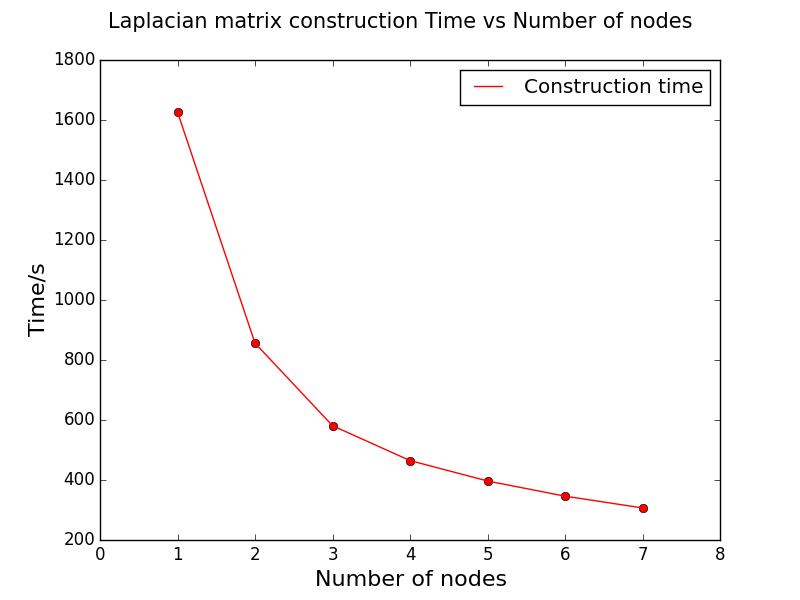
\includegraphics[height=6cm]{mt.png}
\caption{Running time of different optimizations on Musk dataset}
\label{figure_musk_time}
\end{figure}

\begin{figure}
\centering
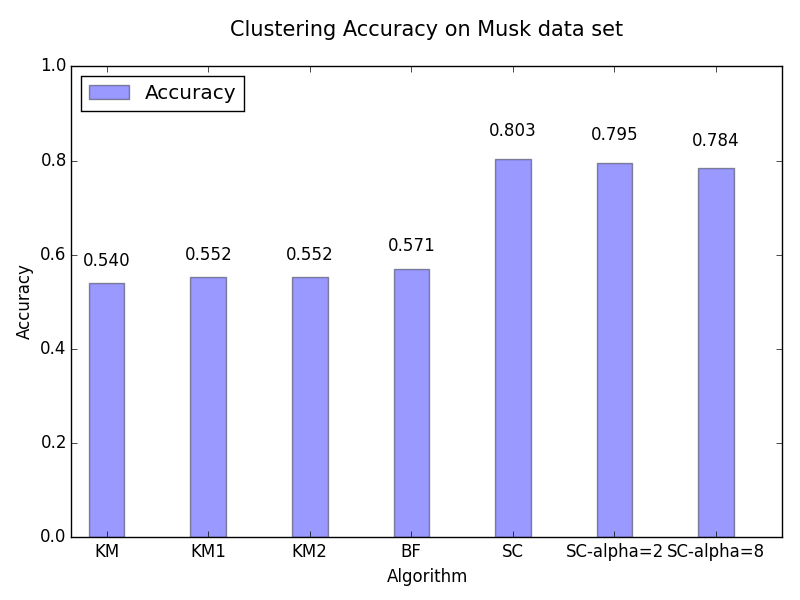
\includegraphics[height=6cm]{ma.png}
\caption{Accuracy of different optimizations on Musk dataset}
\label{figure_musk_accu}
\end{figure}


\begin{table}[h]
\centering
\begin{tabular}{|c|cc|}
\hline
Algorithm & Accuracy & Time \\
\hline
 $k$-means & 0.6325 & 10.50s\\
 SC, $\alpha=500$ & 0.9170 & 141.79s\\
 \hline
\end{tabular}
\caption{Accuracy and running time of $k$-means and spectral clustering settings on USCI dataset}
\label{table_usci}
\end{table}


In Table~\ref{table_usci} we show the accuracy and run time of different clustering algorithms on the USCI dataset. In Figure~\ref{figure_usci_time} we show the run time bar plot of those algorithms and in Figure~\ref{figure_usci_accu} we show the accuracy plot. 

\begin{figure}
\centering
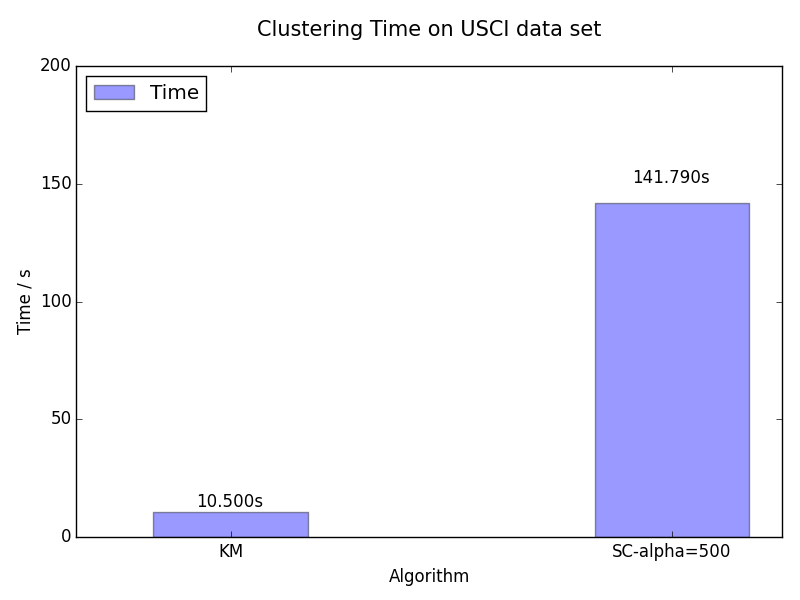
\includegraphics[height=6cm]{ut.png}
\caption{Running time of different optimizations on USCI dataset}
\label{figure_usci_time}
\end{figure}

\begin{figure}
\centering
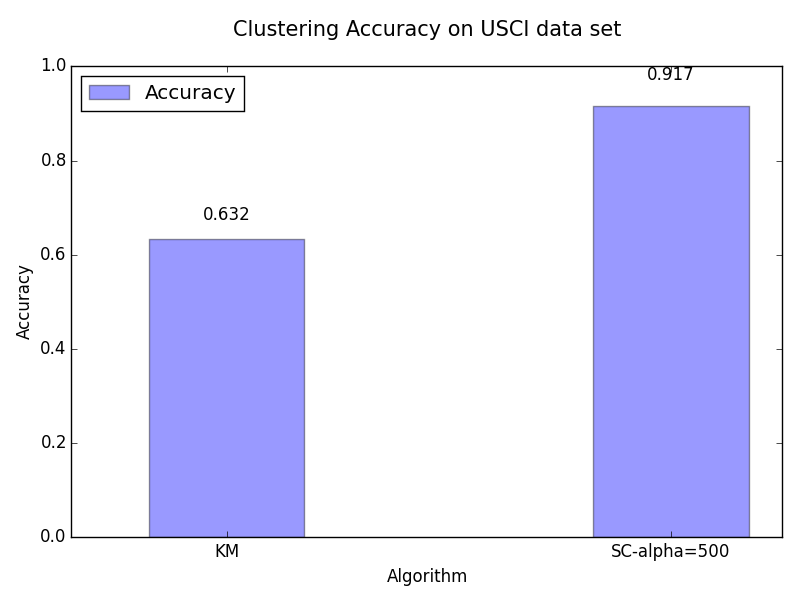
\includegraphics[height=6cm]{ua.png}
\caption{Accuracy of different optimizations on USCI dataset}
\label{figure_usci_accu}
\end{figure}

Since the dataset is huge and it could take days to run the basic Spectral Clustering algorithm, we chose a big downsampling ratio of $\alpha = 500$. The Spectral Clustering is still significantly slower than $k$-means, but gets 0.917 accuracy compared to the 0.6325 from $k$-means.

\section{Conclusion and future work}

In this project we experienced with different clustering algorithms, particularly $k$-means and Spectral Clustering. We tried the basic version of algorithms and different optimization techniques on small and large data set. In short, $k$-means provides a fast clustering centroids searching technique, but the performance depends on the initialization. Spectral Clustering often gives much better results but has memory and runtime bottleneck for large dataset. Applying the downsampling optimization at the beginning would reduce these overheads without losing much accuracies.  

There are lots of potential extension to the project. For example, we could try different similarity metrics, such as Gaussian Kernel, to smooth the distance. We could also use APARPACK to parallelize eigenvalue decomposition. Instead of the simple Laplacian Matrix, we could do a comparison between Spectral Clustering with unnormalized Laplacian matrix and normalized Laplacian matrix.
% The following two commands are all you need in the
% initial runs of your .tex file to
% produce the bibliography for the citations in your paper.
\bibliographystyle{abbrv}
\bibliography{citations}  % sigproc.bib is the name of the Bibliography in this case
% You must have a proper ".bib" file
%  and remember to run:
% latex bibtex latex latex
% to resolve all references
%
% ACM needs 'a single self-contained file'!
%
%APPENDICES are optional
%\balancecolumns

\balancecolumns
% That's all folks!
\end{document}


